% Master's thesis defence — 15 min, widescreen, minimalist design.
% Compile: pdflatex thesis_defense.tex
% Prerequisite: run notebooks/01_EDA.ipynb to regenerate ../plots/eda_brent_events_postcovid.png

\documentclass[aspectratio=169,11pt]{beamer}

% ===== Minimal theme =====
\usetheme{default}
\usecolortheme{default}

% Strip all chrome — no navigation, no symbols, no logos.
\setbeamertemplate{navigation symbols}{}
\setbeamertemplate{headline}{}
\setbeamertemplate{itemize item}{\textbullet}
\setbeamertemplate{itemize subitem}{\textendash}
\setbeamertemplate{itemize subsubitem}{\textperiodcentered}

% Slide number bottom-right, that's it.
\setbeamertemplate{footline}{%
  \hspace*{\fill}\textcolor{gray}{\footnotesize\insertframenumber\,/\,\inserttotalframenumber}\hspace*{1em}\vspace*{0.5em}%
}

% Frame title: regular weight, thin rule below.
\setbeamercolor{frametitle}{fg=black,bg=white}
\setbeamerfont{frametitle}{size=\Large,series=\bfseries}
\setbeamertemplate{frametitle}{%
  \vspace{0.3em}%
  \insertframetitle\par%
  \vspace{0.15em}%
  {\color{black!20}\hrule height 0.4pt}%
  \vspace{0.6em}%
}

% Title page: minimal.
\setbeamerfont{title}{size=\LARGE,series=\bfseries}
\setbeamerfont{subtitle}{size=\large,series=\mdseries,shape=\itshape}
\setbeamerfont{author}{size=\normalsize}
\setbeamerfont{institute}{size=\small,shape=\itshape}
\setbeamercolor{title}{fg=black}
\setbeamercolor{subtitle}{fg=black!70}
\setbeamercolor{author}{fg=black}
\setbeamercolor{institute}{fg=black!60}

% No coloured boxes anywhere.
\setbeamercolor{normal text}{fg=black,bg=white}
\setbeamercolor{structure}{fg=black}

\usepackage{graphicx}
\usepackage{booktabs}
\usepackage{array}
\usepackage{amsmath}
\usepackage{xcolor}

\definecolor{accent}{HTML}{8B0000}      % dark red — used very sparingly
\definecolor{muted}{HTML}{777777}

% Helpers
\newcommand{\src}[1]{{\footnotesize\textcolor{muted}{(#1)}}}
\newcommand{\smalltext}[1]{{\footnotesize\textcolor{muted}{#1}}}
\newcommand{\hd}[1]{\textbf{#1}}

\title{The Brent-Price Causal Effect of the\\ 2026 Hormuz Disruption}
\subtitle{A Synthetic Control Approach}
\author{[Author name]}
\institute{Barcelona School of Economics}
\date{}

\begin{document}

% =====================================================================
% TITLE
% =====================================================================
{\setbeamertemplate{footline}{}
\begin{frame}[plain]
  \vfill
  \begin{center}
    {\LARGE\bfseries The Brent-Price Causal Effect of the\\[0.2em] 2026 Hormuz Disruption}\\[0.8em]
    {\large\itshape A Synthetic Control Approach}\\[2.5em]
    {\normalsize [Author name]}\\[0.3em]
    {\small\itshape\textcolor{muted}{Barcelona School of Economics}}
  \end{center}
  \vfill
\end{frame}
}

% =====================================================================
% 1. From previous — blank
% =====================================================================
\begin{frame}{From the previous presentation}
  \vfill
  \begin{center}
    \textcolor{muted}{\large [ transition recap --- to be added ]}
  \end{center}
  \vfill
\end{frame}

% =====================================================================
% 2. Problem statement + contribution
% =====================================================================
\begin{frame}[shrink=5]{Problem statement \& contribution}
  \footnotesize
  \hd{The question (part 1).}
  \begin{itemize}\setlength\itemsep{0.1em}
    \item Brent price impact of the 2026-02-01 Strait of Hormuz disruption.
    \item Estimand: ATT over a defined post-event window; method: synthetic control on the observed price series.
  \end{itemize}

  \vspace{0.5em}
  \hd{What is new in this research field.}
  \begin{itemize}\setlength\itemsep{0.1em}
    \item No peer-reviewed SCM applied to a crude benchmark for a geopolitical disruption.
    \item Closest mechanical precedent: SCM on Austrian retail fuel \src{Becker, Pfeifer \& Schweikert 2021, \textit{Energy Economics}}.
    \item Field default: structural VAR \src{Kilian 2009; Baumeister \& Hamilton 2019} or scenario models (Dallas Fed, OIES, Kiel, IEA).
  \end{itemize}

  \vspace{0.5em}
  \hd{Contribution and value.}
  \begin{itemize}\setlength\itemsep{0.1em}
    \item Data-driven counterfactual complements scenario estimates.
    \item Method extension: retail fuel $\rightarrow$ crude benchmark; cross-country $\rightarrow$ cross-asset donors; regulatory $\rightarrow$ exogenous geopolitical treatment.
    \item Policy inputs: SPR sizing, central-bank reaction, fiscal buffers, sovereign hedging, infrastructure investment.
  \end{itemize}

  \vspace{0.5em}
  \hd{Part 2 of the thesis.} \textcolor{muted}{[ discussed at the end ]}
\end{frame}

% =====================================================================
% 3. Historical Brent + events
% =====================================================================
\begin{frame}{???}
  \begin{center}
    \includegraphics[width=0.95\textwidth,height=0.80\textheight,keepaspectratio]{../plots/eda_brent_events_postcovid.png}
  \end{center}
  \vspace{-0.3em}
  \begin{center}
    \smalltext{Brent spot, post-COVID. Events: demand (blue), supply (red), policy (purple), geopolitics (orange).}
  \end{center}
\end{frame}

% =====================================================================
% 4. Methodology — 5 models
% =====================================================================
\begin{frame}{Methodology --- ensemble of 5 models}
  \footnotesize
  \hd{Why an ensemble.} Headline = median across models; IQR = model-uncertainty band.

  \vspace{0.4em}
  \begin{tabular}{@{}p{0.20\textwidth} p{0.40\textwidth} p{0.34\textwidth}@{}}
    \toprule
    \hd{Model} & \hd{What it does} & \hd{Reference} \\
    \midrule
    Convex SCM     & Convex weights, no extrapolation                    & Abadie, Diamond \& Hainmueller (2010, \textit{JASA}) \\
    Augmented SCM  & Convex + ridge bias correction                      & Ben-Michael, Feller \& Rothstein (2021, \textit{JASA}) \\
    Elastic-net    & $L_1 + L_2$ regression, sparse donor weights        & Doudchenko \& Imbens (2016, NBER WP) \\
    XGBoost        & Gradient-boosted trees, flexible nonlinear          & Chen \& Guestrin (2016, \textit{KDD}) \\
    Bayesian Ridge & Bayesian linear with normal prior, donor PIPs       & Tipping (2001); Brodersen et al.\ (2015) \\
    \bottomrule
  \end{tabular}

  \vspace{0.4em}
  \hd{Range covered.} Convex (no extrap) $\rightarrow$ augmented (ridge fix) $\rightarrow$ regression (sparse) $\rightarrow$ nonlinear $\rightarrow$ Bayesian (uncertainty).
\end{frame}

% =====================================================================
% 4b. Model setup --- windows, walk-forward CV, final refit
% =====================================================================
\begin{frame}[shrink=5]{Model setup}
  \footnotesize
  \begin{tabular}{@{}l l l@{}}
    \toprule
                       & \hd{Pre-event window (walk-forward CV)}              & \hd{Treatment (post)} \\
    \midrule
    \hd{Russia 2022}   & 2020-07-01 $\rightarrow$ 2022-02-23 \quad 421 obs    & 2022-02-24 $\rightarrow$ 2022-09-30 \quad 151 obs \\
    \addlinespace
    \hd{Hormuz 2026}   & 2024-06-03 $\rightarrow$ 2026-01-30 \quad 423 obs    & 2026-02-01 $\rightarrow$ 2026-05-01 \quad $\sim$59 obs \\
    \bottomrule
  \end{tabular}
  \normalsize

  \vspace{0.5em}
  \hd{Hyperparameter tuning --- multi-fold walk-forward CV.}
  \begin{itemize}\setlength\itemsep{0.08em}
    \item 5 expanding-window folds inside the pre-event period; 20-bday horizon per fold.
    \item Pick hparams by pooled val RMSE \src{Hyndman \& Athanasopoulos 2018 \S5.10}.
    \item Final fit refits on full pre-event window, projects through treatment.
  \end{itemize}

  \vspace{0.4em}
  \hd{Limitation.} No held-out test set beyond train/val; generalisation to unseen data cannot be measured directly. Formal inference $\rightarrow$ in-space placebo.
\end{frame}

% =====================================================================
% 5. Validation — minimum load-bearing
% =====================================================================
\begin{frame}{Validation }

  \vspace{0.6em}
  \hd{1. Model fit.} \smalltext{Is the synthetic a credible pre-event approximator?}
  \begin{itemize}\setlength\itemsep{0.15em}
    \item Walk-forward CV \src{Hyndman \& Athanasopoulos 2018; Bergmeir \& Benítez 2012}.
  \end{itemize}

  \vspace{0.5em}
  \hd{2. Donor identification.} \smalltext{Are the donors statistically clean of the event (SUTVA)?}
  \begin{itemize}\setlength\itemsep{0.15em}
    \item Qualitative audit on causal channels \src{Abadie 2021 \S3.1}.
    \item Bootstrap structural break at $T_0$ \src{Andrews 1993; Hansen 2000}.
  \end{itemize}

  \vspace{0.5em}
  \hd{3. Inference.} \smalltext{Is the post-event gap larger than under the no-treatment null?}
  \begin{itemize}\setlength\itemsep{0.15em}
    \item In-space placebo, 21- and 33-donor pools \src{Abadie 2010 \S3.3}.
    \item Cross-event weight transfer --- Hormuz only, substitutes for the low-power placebo at $\sim$60 post-event obs.
  \end{itemize}
\end{frame}

% =====================================================================
% 6. Donor selection
% =====================================================================
\begin{frame}{Donor selection}
  \hd{21 audited donors.} Inclusion requires \emph{both}: \hd{pre-treatment} co-movement with Brent through a common global factor, \emph{and} \hd{treatment} cleanliness (no Russia/Ukraine or Persian Gulf exposure --- SUTVA).

  \vspace{0.4em}
  \scriptsize
  \begin{tabular}{@{}p{0.16\textwidth} p{0.30\textwidth} p{0.46\textwidth}@{}}
    \toprule
    \hd{Category}      & \hd{Chosen donors}                                & \hd{Factor channel (pre) \& cleanliness (treatment)} \\
    \midrule
    Metals (3)         & Silver, Platinum, Gold                            & Real rates / safe-haven / auto industry; no Russia or Gulf supply routing. \\
    Agriculturals (4)  & Coffee, Sugar, Cotton, LiveCattle                 & Global trade activity (Brazil / India / US producers); outside the Russia-Ukraine grain belt. \\
    Equities (3)       & SP500, WorldEq, Nikkei                            & Global growth / equity risk premium; no direct Russia or Gulf-energy exposure. \\
    FX (8)             & AUD, JPY, CHF, CNY, INR, KRW, ZAR, MXN            & Safe-haven, EM growth, China demand; no petrocurrency or EU-energy-crisis loading. \\
    Rates / credit (2) & TLT, HYG                                          & US duration / credit-risk premia; not directly oil-linked. \\
    Volatility (1)     & VIX                                               & S\&P 500 implied vol --- risk-on/off via equities. \\
    \bottomrule
  \end{tabular}
  \normalsize

  \vspace{0.4em}
  \smalltext{Categorical exclusions and per-event flag table: docs/donor\_catalog.md.}
\end{frame}

% =====================================================================
% 7. Donor co-movement with Brent --- side-by-side
% =====================================================================
\begin{frame}{Donor co-movement with Brent --- audited pool}
  \begin{center}
    \includegraphics[width=0.85\textwidth,height=0.72\textheight,keepaspectratio]{../plots/eda_donors_audited_side_by_side.png}\\[0.1em]
    \smalltext{Brent (black) vs 21 audited donors, rebased to 100 at pre-window start; dashed line marks $T_0$. Same windows as the SCM.}
  \end{center}
\end{frame}

% =====================================================================
% 8. Validation results — model fit
% =====================================================================
\begin{frame}{Validation results --- model fit}
  \begin{center}
    
\includegraphics[width=0.90\textwidth,height=0.56\textheight,keepaspectratio]{../plots/ensemble/ensemble_paths_side_by_side.png}
  \end{center}

  \vspace{-0.1em}
  \begin{center}
  \tiny
  \begin{tabular}{@{}l r r r r@{}}
    \toprule
    \hd{Model}     & \hd{Russia train} & \hd{Russia val} & \hd{Hormuz train} & \hd{Hormuz val} \\
    \midrule
    Convex SCM     & 0.111 & 0.086 & 0.059 & 0.129 \\
    ASCM           & 0.046 & 0.087 & 0.035 & 0.087 \\
    Elastic-net    & 0.055 & 0.094 & 0.043 & 0.049 \\
    XGBoost        & 0.039 & 0.135 & 0.045 & 0.089 \\
    Bayesian Ridge & 0.034 & 0.171 & 0.033 & 0.093 \\
    \bottomrule
  \end{tabular}
  \normalsize
  \end{center}
\end{frame}

% =====================================================================
% 8. Donor importance
% =====================================================================
\begin{frame}{Donor importance}
  \begin{center}
    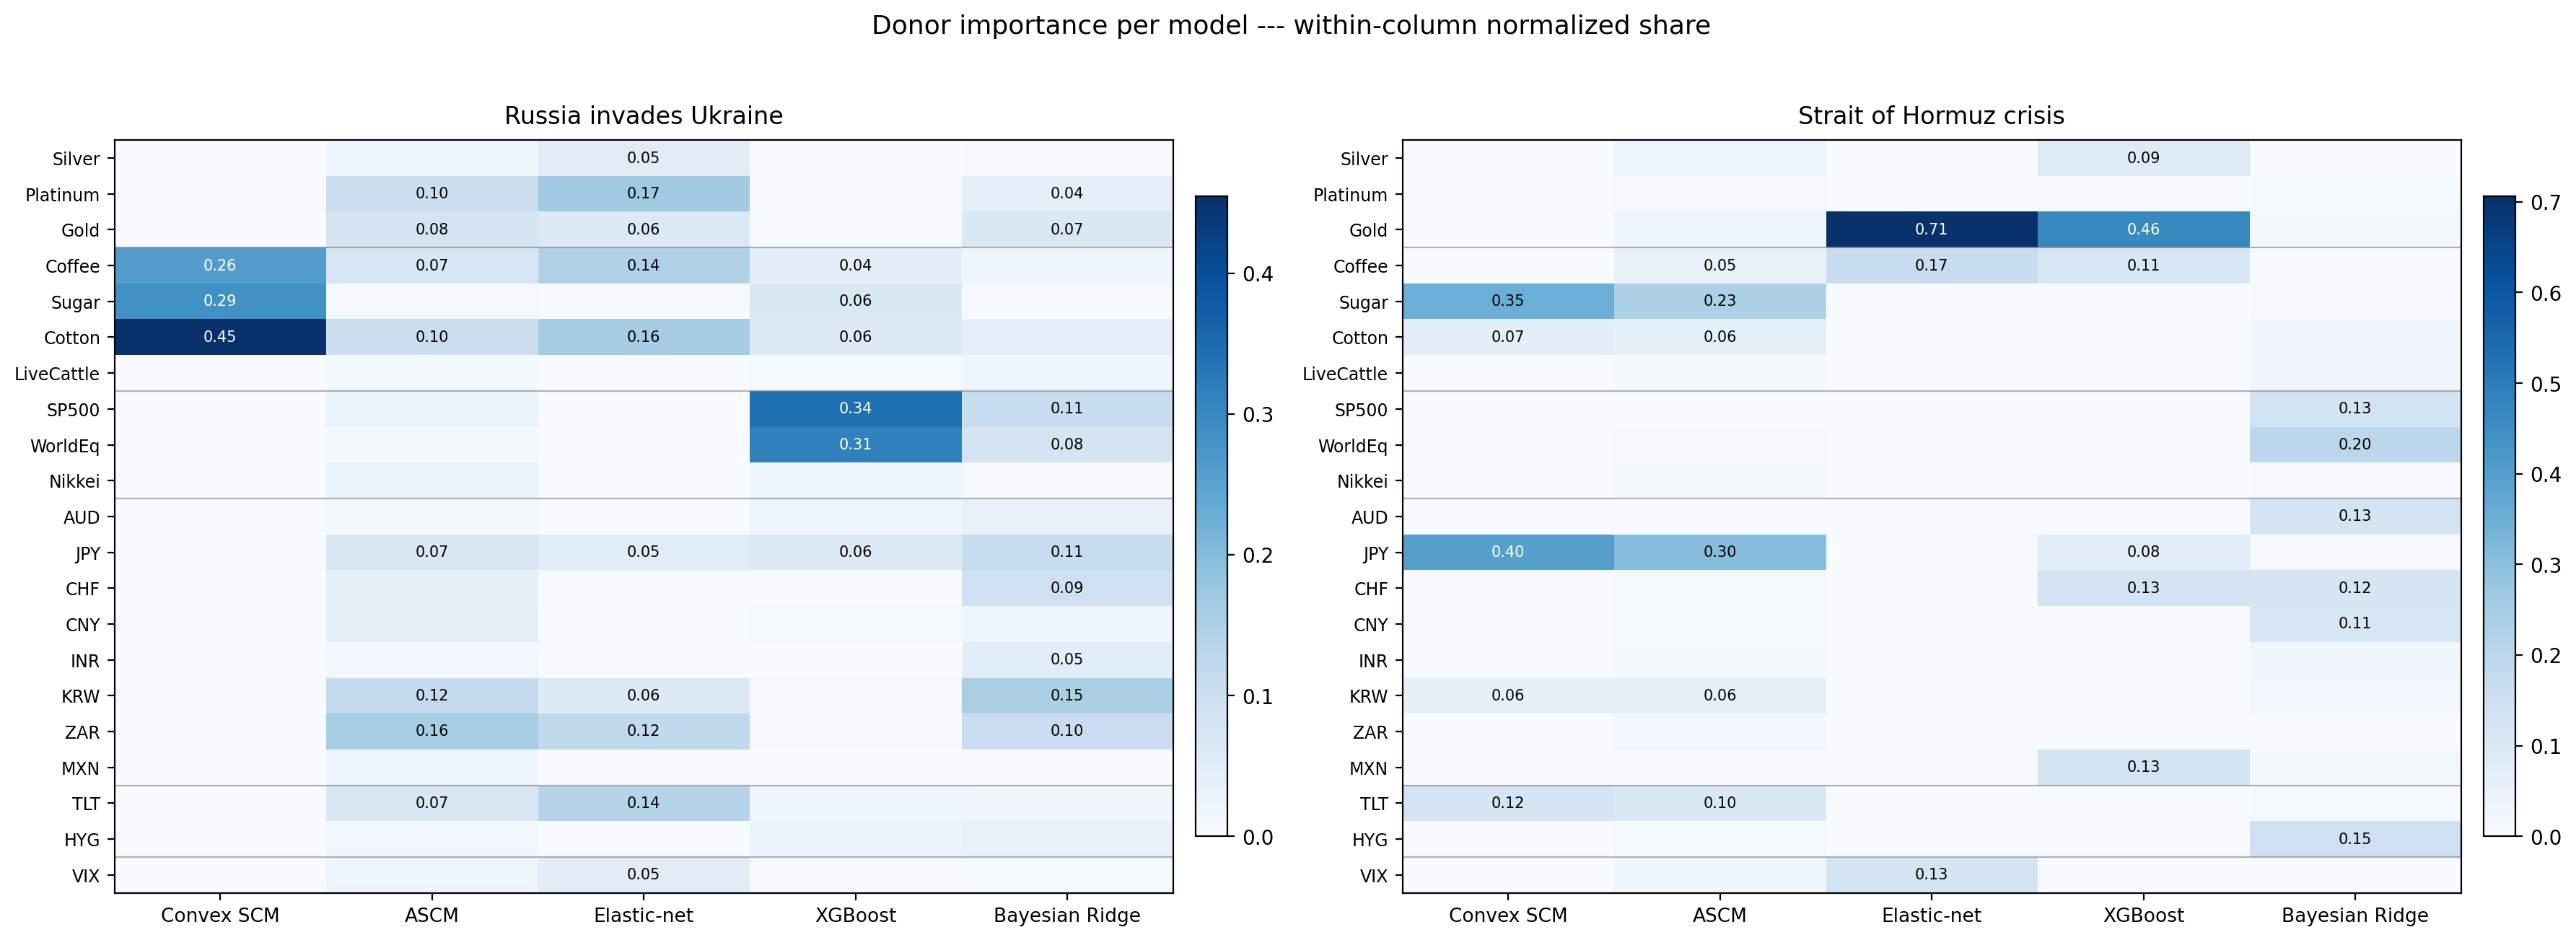
\includegraphics[width=0.98\textwidth,height=0.72\textheight,keepaspectratio]{../plots/milestone2/donor_importance_heatmap.png}
  \end{center}

  \vspace{-0.1em}
  \begin{center}
  {\scriptsize\textcolor{muted}{Per-model raw metric: convex weight $w_j$ (SCM, ASCM) / $|\hat\beta_j|$ (Elastic-net, Bayesian Ridge) / feature importance (XGBoost). Cells $= |w_j|$ normalised within each column to sum to 1.}}
  \end{center}
\end{frame}

% =====================================================================
% 9. Validation results — in-space placebo
% =====================================================================
\begin{frame}{Validation results --- in-space placebo}
  \hd{Abadie's canonical test} \src{Abadie 2010 \S3.3}: rank Brent's post/pre RMSPE ratio against the placebo distribution.

  \vspace{0.6em}
  \hd{Two donor pools for resolution.}
  \begin{itemize}\setlength\itemsep{0.1em}
    \item Shared 21-donor preferred: $p$-floor $= 1/22 \approx 0.045$.
    \item Full 33-donor pool: $p$-floor $= 1/34 \approx 0.029$.
  \end{itemize}

  \vspace{0.6em}
  \hd{Headline.}

  \vspace{0.3em}
  \begin{tabular}{@{}p{0.20\textwidth} p{0.30\textwidth} p{0.30\textwidth}@{}}
    \toprule
                  & \hd{Russia 2022} & \hd{Hormuz 2026} \\
    \midrule
    21-donor      & \textcolor{muted}{[ $p$ ]} & \textcolor{muted}{[ $p$ ]} \\
    33-donor      & \textcolor{muted}{[ $p$ ]} & \textcolor{muted}{[ $p$ ]} \\
    \bottomrule
  \end{tabular}

  \vspace{0.5em}
  \smalltext{Everything else (parallel-fit, regime-stability, in-time placebo, LOO, cross-event transfer): appendix.}
\end{frame}

% =====================================================================
% 9b. External validation — EIA STEO pre-invasion forecasts (Russia only)
% =====================================================================
\begin{frame}{External validation --- EIA STEO pre-invasion forecasts (Russia only)}
  \hd{Cross-method check.} SCM counterfactual vs EIA's last pre-invasion Brent forecast (STEO Feb-22, issued 2022-02-08). No shared information path (SCM uses cross-assetco-movement; STEO uses fundamental supply-demand modelling)

  \vspace{0.6em}
  \footnotesize
  \begin{tabular}{@{}l r r r@{}}
    \toprule
    \hd{Model}     & \hd{Synth \$/bbl} & \hd{STEO Feb-22 \$/bbl} & \hd{$\Delta$} \\
    \midrule
    Convex SCM     & 83.55             & 84.94                   & $-$\$1.39  \\
    ASCM           & 95.52             & 84.94                   & $+$\$10.58 \\
    Elastic-net    & 86.61             & 84.94                   & $+$\$1.67  \\
    XGBoost        & 79.37             & 84.94                   & $-$\$5.57  \\
    Bayesian Ridge & 107.91            & 84.94                   & $+$\$22.97 (deg.) \\
    \midrule
    \hd{Ensemble median} & \hd{86.61}  & \hd{84.94}              & \hd{$+$\$1.67} \\
    \bottomrule
  \end{tabular}
  \normalsize

  \vspace{0.6em}
  \hd{Implied ATT} \smalltext{(Brent actual \$108.54)}: SCM ensemble $+$25.3\% \quad vs \quad STEO Feb-22 $+$27.8\% \quad ($\Delta \sim$ 2.5 pp).

  \vspace{0.3em}
\end{frame}

% =====================================================================
% 10. ATT estimate
% =====================================================================
\begin{frame}[shrink=5]{Headline result --- ATT estimate}
  \hd{ATT (\% log Brent) over the post-event window.}

  \vspace{0.6em}
  \begin{tabular}{@{}l c c@{}}
    \toprule
    \hd{Model}     & \hd{Russia 2022} & \hd{Hormuz 2026} \\
                   & \smalltext{(2022-02-24 $\rightarrow$ 2022-09-30)} & \smalltext{(2026-02-01 $\rightarrow$ latest)} \\
    \midrule
    Convex SCM         & \textcolor{muted}{[ \% ]} & \textcolor{muted}{[ \% ]} \\
    ASCM               & \textcolor{muted}{[ \% ]} & \textcolor{muted}{[ \% ]} \\
    Elastic-net        & \textcolor{muted}{[ \% ]} & \textcolor{muted}{[ \% ]} \\
    XGBoost            & \textcolor{muted}{[ \% ]} & \textcolor{muted}{[ \% ]} \\
    Bayesian Ridge     & \textcolor{muted}{[ \% ]} & \textcolor{muted}{[ \% ]} \\
    \midrule
    \hd{Ensemble median} & \textcolor{accent}{\hd{[ \% ]}} & \textcolor{accent}{\hd{[ \% ]}} \\
    IQR                & \textcolor{muted}{[ band ]} & \textcolor{muted}{[ band ]} \\
    \bottomrule
  \end{tabular}

  \vspace{0.6em}
  \hd{Reading.}
  \begin{itemize}\setlength\itemsep{0.05em}
    \item Russia: calibration case; compare to documented \$95 $\rightarrow$ \$130+ move.
    \item Hormuz: main thesis result; place against scenario estimates (Dallas Fed, OIES, IEA).
  \end{itemize}
\end{frame}

% =====================================================================
% 11. Part 2
% =====================================================================
\begin{frame}{Part 2 --- ideas for the second half}
  \vfill
  \begin{center}
    \textcolor{muted}{\large [ to be added by author ]}
  \end{center}

  \vspace{1.5em}
  \begin{center}
    \smalltext{Possible directions: pass-through to retail fuel / headline CPI; SCM vs scenario-model comparison; severity-dependent extrapolation; alternative donor pools.}
  \end{center}
  \vfill
\end{frame}

% =====================================================================
% Closing
% =====================================================================
{\setbeamertemplate{footline}{}
\begin{frame}[plain]
  \vfill
  \begin{center}
    {\Large Thank you}\\[1em]
    {\normalsize Questions and discussion}\\[2em]
    \smalltext{github.com/ElvisCasco/Brent\_Analysis}
  \end{center}
  \vfill
\end{frame}
}

\end{document}
